\documentclass[border=6pt,tikz]{standalone}
\usepackage{tikz}
\usepackage{amsmath,amssymb}
\usetikzlibrary{arrows.meta,positioning,fit,backgrounds,calc,shapes.geometric,decorations.pathreplacing,patterns}
\definecolor{ink}{HTML}{1B2430}
\definecolor{muted}{HTML}{6B7785}
\definecolor{accent}{HTML}{2F6FB5}
\definecolor{accent2}{HTML}{C1611F}
\definecolor{good}{HTML}{2E7D5B}
\definecolor{soft}{HTML}{EDF2F7}
\definecolor{soft2}{HTML}{FBEDE2}
\definecolor{soft3}{HTML}{E6F0E9}
\tikzset{
  box/.style={draw=ink,line width=.7pt,rounded corners=2pt,fill=soft,inner sep=4pt,align=center,font=\sffamily\small},
  boxa/.style={box,fill=soft2},
  boxb/.style={box,fill=soft3},
  plain/.style={align=center,font=\sffamily\small,text=ink},
  tiny/.style={align=center,font=\sffamily\scriptsize,text=muted},
  ar/.style={-{Stealth[length=2.4mm]},draw=ink,line width=.7pt},
  arm/.style={-{Stealth[length=2.4mm]},draw=muted,line width=.6pt,dashed},
  nd/.style={circle,draw=ink,line width=.7pt,fill=white,minimum size=7mm,inner sep=0pt,font=\sffamily\scriptsize},
  ndf/.style={nd,fill=soft},
  ndt/.style={nd,fill=soft2},
}

\begin{document}
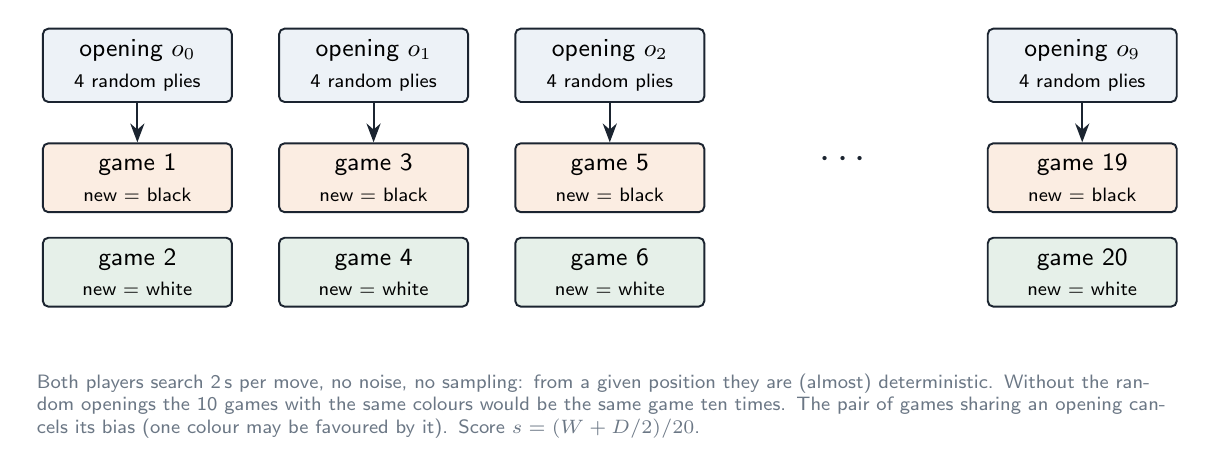
\begin{tikzpicture}[x=1mm,y=1mm]
  \foreach \p/\x in {0/0,1/30,2/60} {
    \pgfmathtruncatemacro{\ga}{2*\p+1}\pgfmathtruncatemacro{\gb}{2*\p+2}
    \node[box,minimum width=24mm] (o\p) at (\x,0) {opening $o_{\p}$\\\scriptsize 4 random plies};
    \node[boxa,minimum width=24mm,below=5mm of o\p] (a\p) {game \ga\\\scriptsize new = black};
    \node[boxb,minimum width=24mm,below=3mm of a\p] (b\p) {game \gb\\\scriptsize new = white};
    \draw[ar] (o\p) -- (a\p);
  }
  \node[plain] at (90,-12) {\Large$\cdots$};
  \node[box,minimum width=24mm] (o9) at (120,0) {opening $o_{9}$\\\scriptsize 4 random plies};
  \node[boxa,minimum width=24mm,below=5mm of o9] (a9) {game 19\\\scriptsize new = black};
  \node[boxb,minimum width=24mm,below=3mm of a9] (b9) {game 20\\\scriptsize new = white};
  \draw[ar] (o9) -- (a9);
  \node[tiny,text width=145mm,align=left,anchor=north west] at (-14,-38)
  {Both players search 2\,s per move, no noise, no sampling: from a given position they are (almost) deterministic.
   Without the random openings the 10 games with the same colours would be the same game ten times. The pair of
   games sharing an opening cancels its bias (one colour may be favoured by it). Score $s=(W+D/2)/20$.};
\end{tikzpicture}
\end{document}
